\section{User Interaction\label{sec:interaction}}
\begin{figure}[ht!]
\centering
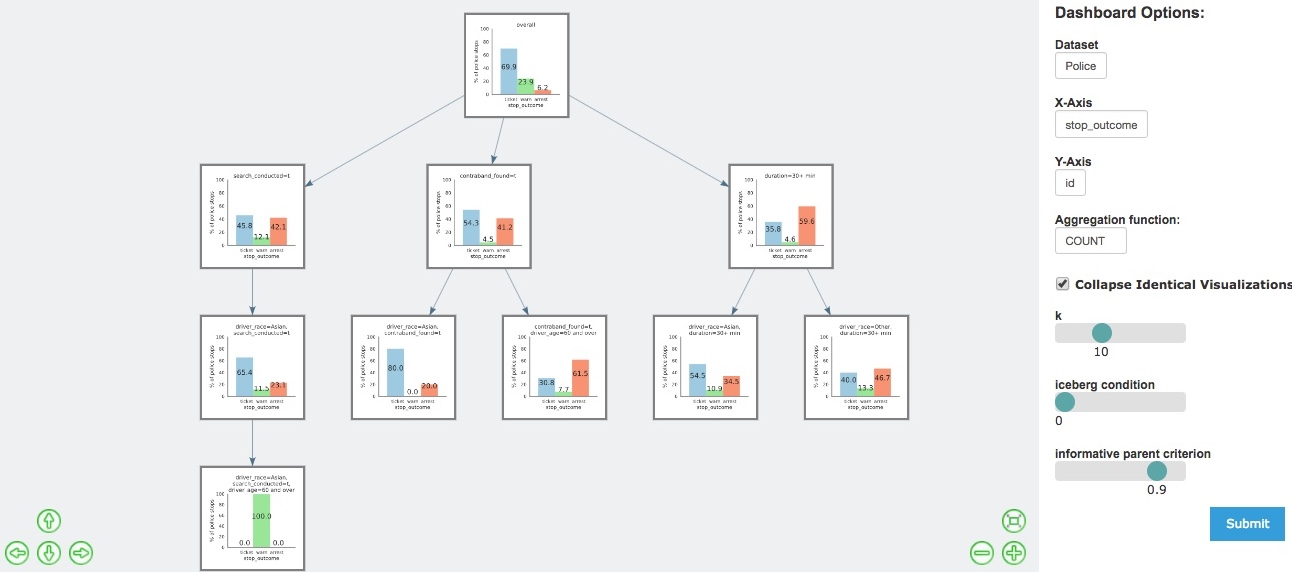
\includegraphics[width=\linewidth]{figures/overview.jpeg}
\caption{Overview of the \system interface for the Police Dataset~\cite{ctrp3}. Users can select x and y axes of interest, as well as a choice of an aggregation function. Default values are set for system related parameters such as the number of visualizations to show in the dashboard (k), iceberg condition for pruning ($\delta$), and informative parent criterion ($\theta$), which can be adjusted by the users via the sliders if needed.}
\label{fig:overview}
\end{figure}
\par Figure \ref{fig:overview} shows an overview of the \system interface. After the user selects the x and y axes of interest, aggregation function, and optional system parameter settings, an initial dashboard of $k$ visualizations is displayed on the canvas, such as the one seen in main canvas of Figure \ref{fig:overview}.  The system provides toolbar buttons with keyboard binding for zooming in, out, and extent, as well as moving around the canvas. Alternatively, users can zoom and pan with mouse click and scroll.

%\hdev{(1) The second sentence is in passive voice. (2) What are the optional system parameters? Clearly state them. (1) Simplify the third sentence. A non-UI person may not know the meaning of some of the terms. (1) In fourth sentence, if you are using "alternatively", there's no need for "also".}

\par After browsing through the visualizations in the dashboard, users may be interested in getting more information about a particular node. \system supports a mechanism for users to request additional summarizations based on a chosen visualization of interest. As shown in Figure \ref{fig:altroot_expansion} (left), the analyst starts with a 5-visualization dashboard on a police stop dataset~\cite{ctrp3}. The dataset contains  records of vehicle and pedestrian stops from law enforcement departments in Connecticut, dated from 2013 to 2015. The analyst learns that for the drivers who had contraband found in the vehicle, the arrest rate for drivers who are 60 and over is surprisingly higher than usual, whereas for Asian drivers the arrest rate is lower. In addition, he is also interested in learning more about the other factor that contribute to high arrest rate: duration=30+min. He clicks on the corresponding visualization and requests for 2 additional visualizations. Upon seeing the updated dashboard in Figure~\ref{fig:altroot_expansion} (right), he learns that similar to the selected visualization, any visualization that involves the duration=30+min filter results in high ticketing and arrest rates. This implies that if a police stop lasts more than 30 minutes, the outcome would more or less be the same, independent of other factors, such as driver's race or age. \system uses the same models and algorithms as before, except the root node is now set as the selected visualization, rather than the overall visualization. This node expansion capability is similarly motivated by the idea of \textit{iterative view refinement} in other visual analytics system \cite{Wongsuphasawat2016,Hoque2017}, which is essential for the users to iterate on and explore different hypotheses.

\begin{figure}[ht!]
\centering
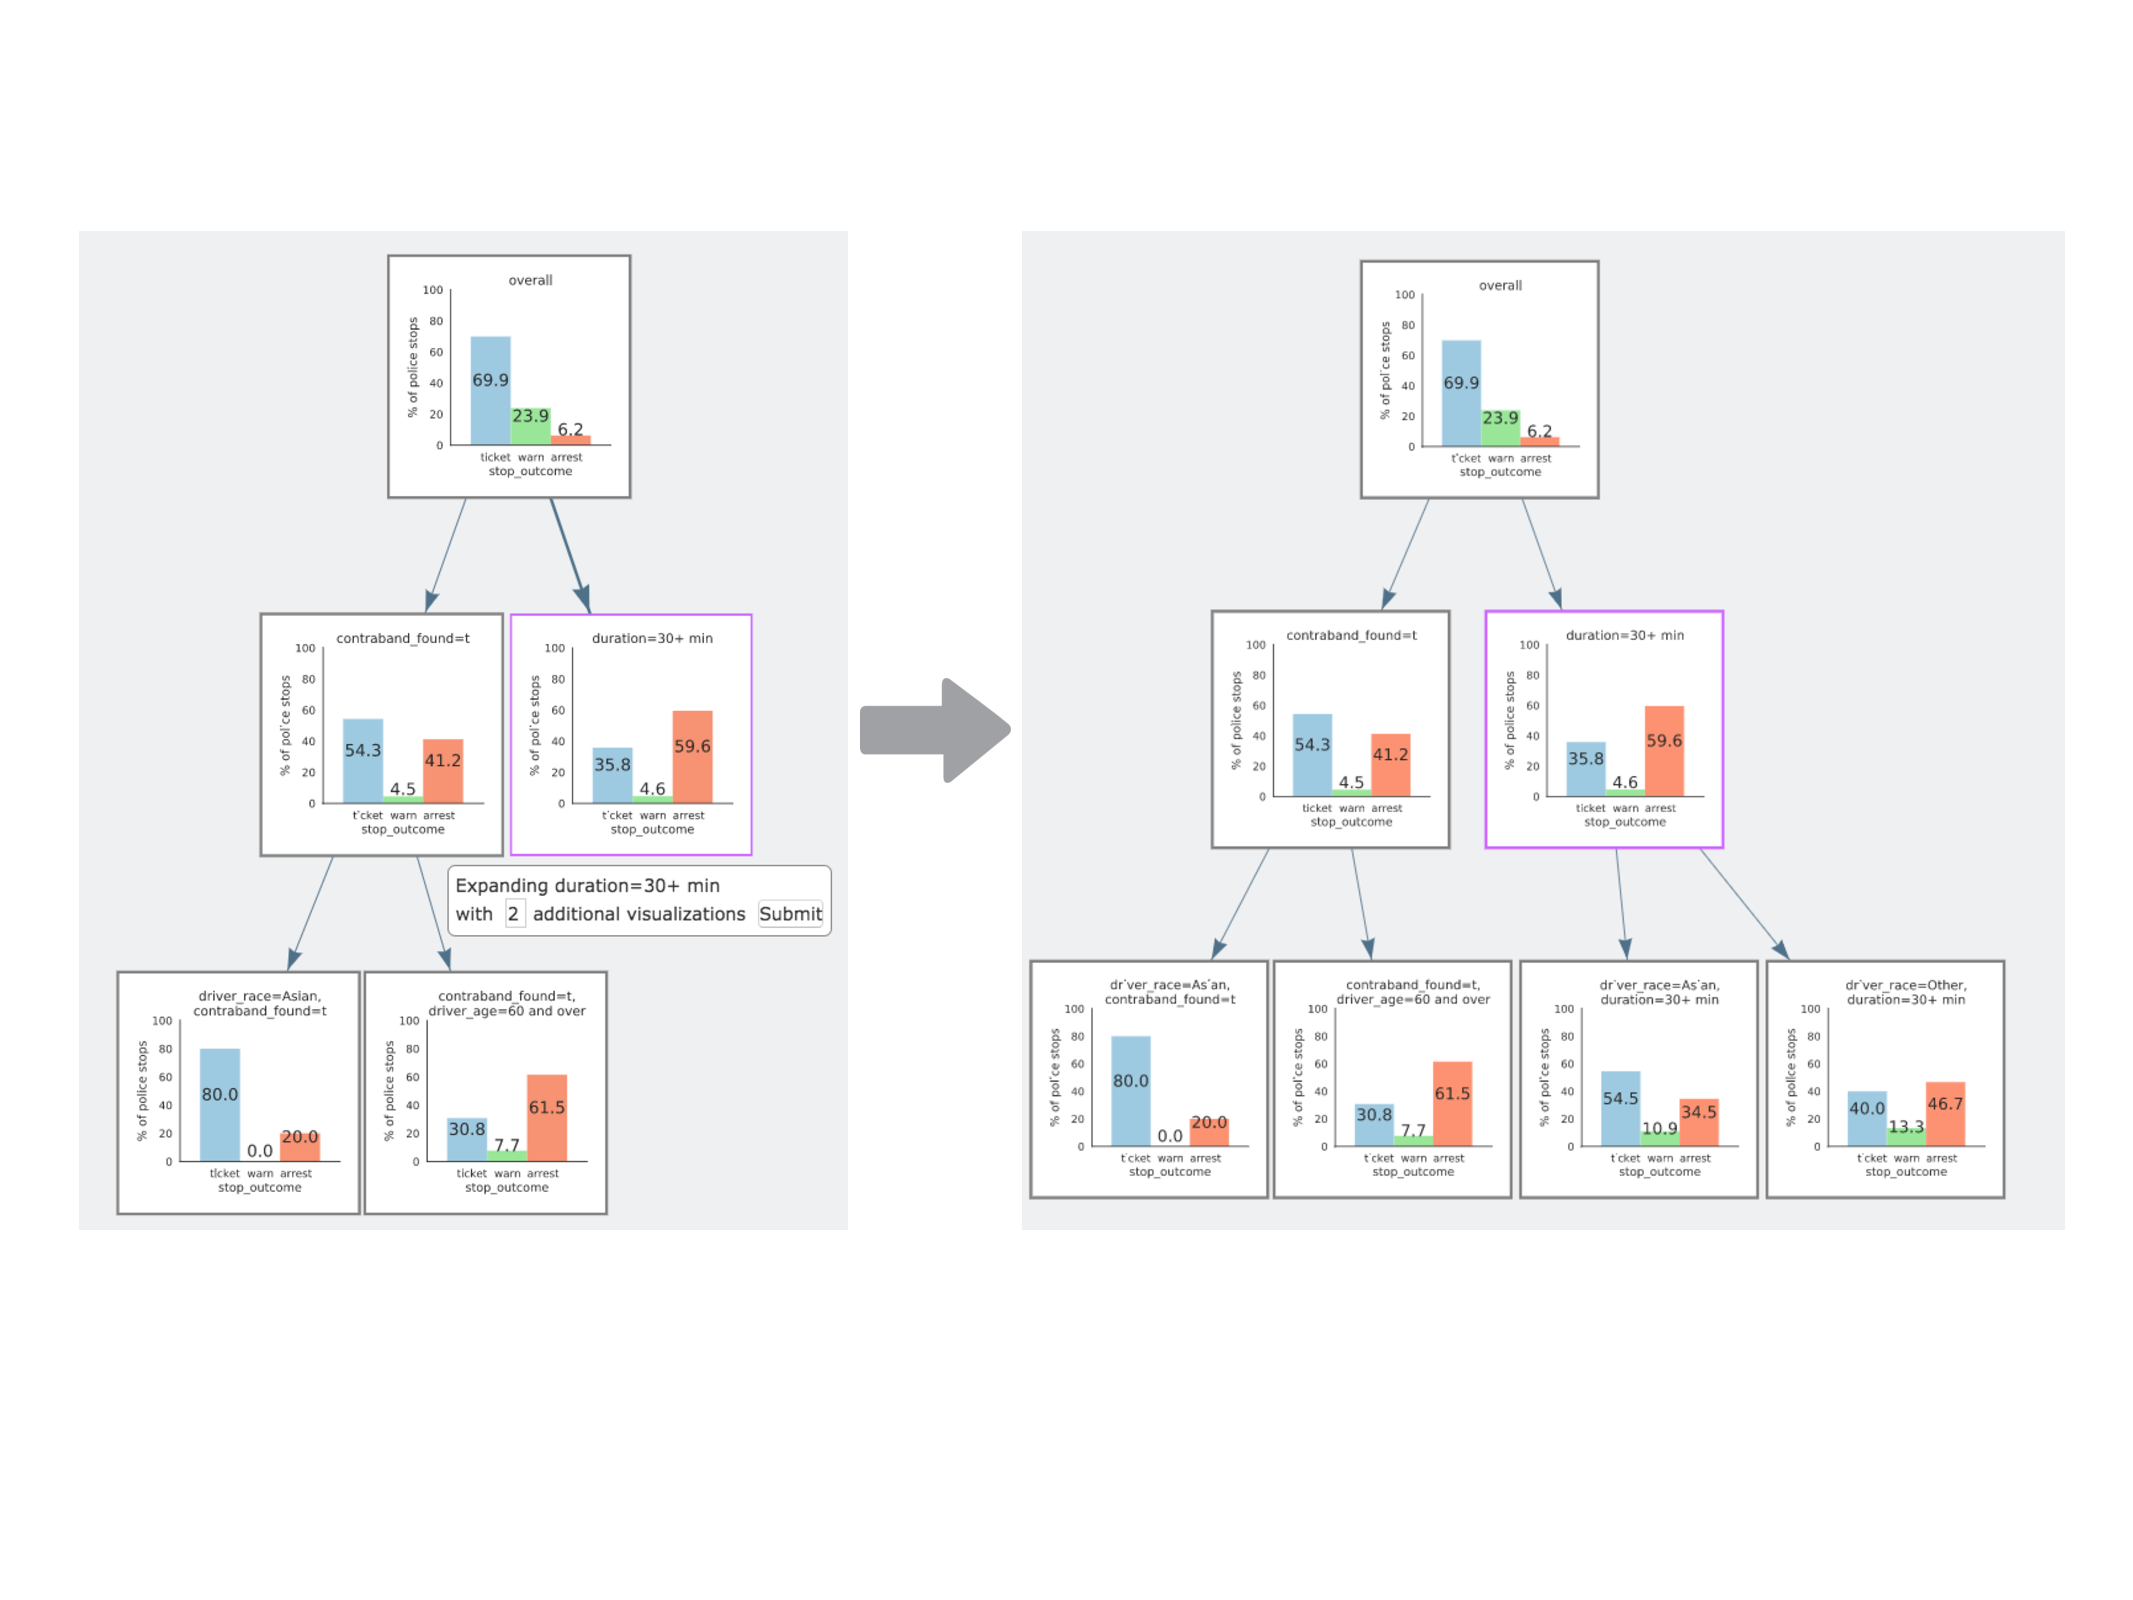
\includegraphics[width=\linewidth]{figures/expansion_example.pdf}
\caption{Left: Original k=5 dashboard with the duration=30+min visualization clicked. A pop-up is displayed to submit the request for additional summary visualizations to be generated. Right: Resulting dashboard after requesting for 2 more visualizations based on the visualization of interest.}
\label{fig:altroot_expansion}
\end{figure}

\subsection{Assistive tools for visualizing large lattices\label{sec:navigation}}
Due to the amount of space occupied by the hierarchical layout when the number of visualizations gets large, we have developed tools to help users navigate through different parts of the dashboard interactively.
\stitle{Navigation Minimap:}  When the user zooms in on the dashboard, an overview mini-map is shown on the upper left-hand side of the canvas to help users identify which region of the dashboard they are currently exploring, as shown in Figure \ref{fig:hover_minimap}.
\stitle{Collapsed visualizations:}
One observation that we found across several datasets was that many visualizations had identical distributions, which resulted in lots of wasted space. Apart from their attribute name, these visualizations are not very informative for the users, therefore, we offer an option to collapse these visualization, as demonstrated in Figure \ref{fig:collapse_demo}. A visualization can be collapsed if it has more than one redundant sibling and does not have any children, so that there are no hidden stories due to lower-level dependencies. As shown in Figure \ref{fig:hover_minimap}, collapsed nodes can be easily identified by an orange border and the details of which visualizations are in the collapsed node are displayed when the user hovers over the visualization.
%\afterpage{%to enable footnote in caption
\begin{figure}[ht!]
\centering
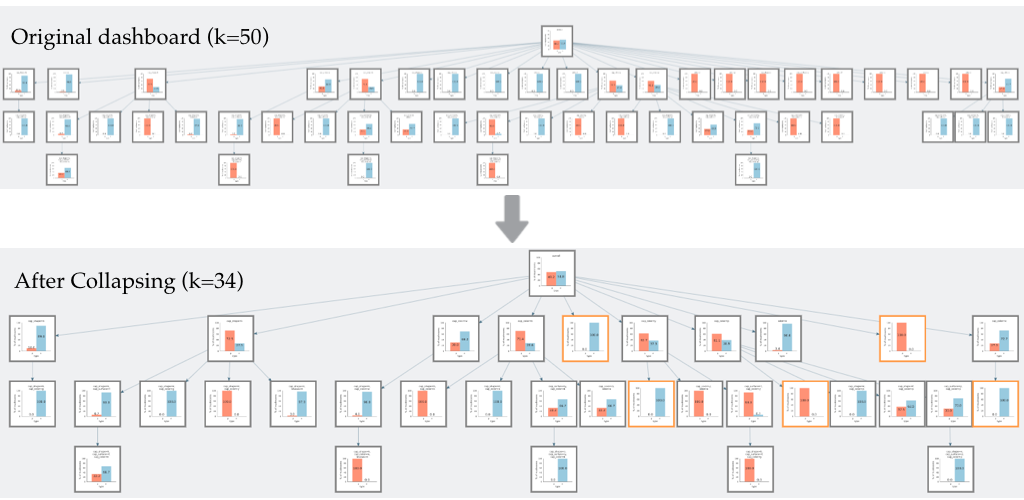
\includegraphics[width=\linewidth]{figures/collapsed_example.png}
\caption{An example of the k=50 dashboard for the mushroom dataset\cite{mushroom}, which contains type=\{posionous, edible\} on the x-axis. The collapsed dashboard (bottom) removed 16 redundant visualizations from the original dashboard (top).}
\label{fig:collapse_demo}
\end{figure}
%}
\begin{figure}[ht!]
\centering
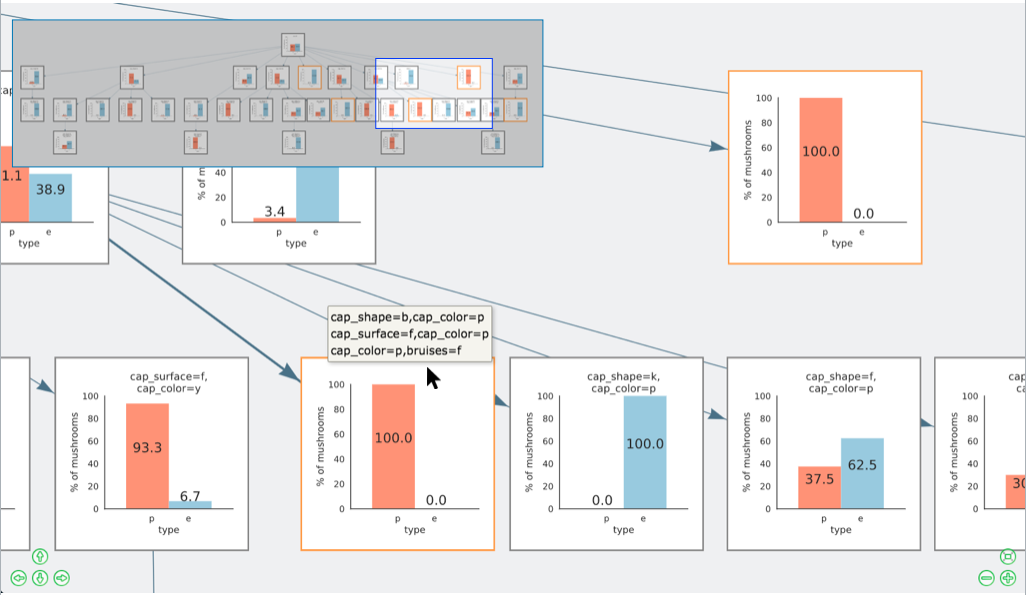
\includegraphics[width=\linewidth]{figures/minimap_zoom.png}
\caption{Zoomed-in version of Figure \ref{fig:collapse_demo} showing the labels of a collapsed visualization when user hovers over the visualization. The navigation minimap is shown in the top-left to help users navigate through the large dashboard.}
\label{fig:hover_minimap}
\end{figure}
